% !TEX root = ../../../semexp-thesis.tex

\section{Domain Model}
\label{sec:semtex/model}

We describe our domain model of semantic technologies for programming semantic searches and conversational agents.

\subsection*{Semantic Search}
\label{sec:semtex/model/search}

To model semantic search in the context of the Squeak ecosystem, \semtex defines the central class \code{SemanticCorpus} as a specialization of the \code{Set} class from the Collections package~(\cref{fig:semtex/model/search}).
This class extends the responsibilities of a regular collection for containing any number of (domain) objects with those of a vector store for searching and filtering objects based on document embeddings.

\begin{figure}
	\centering
	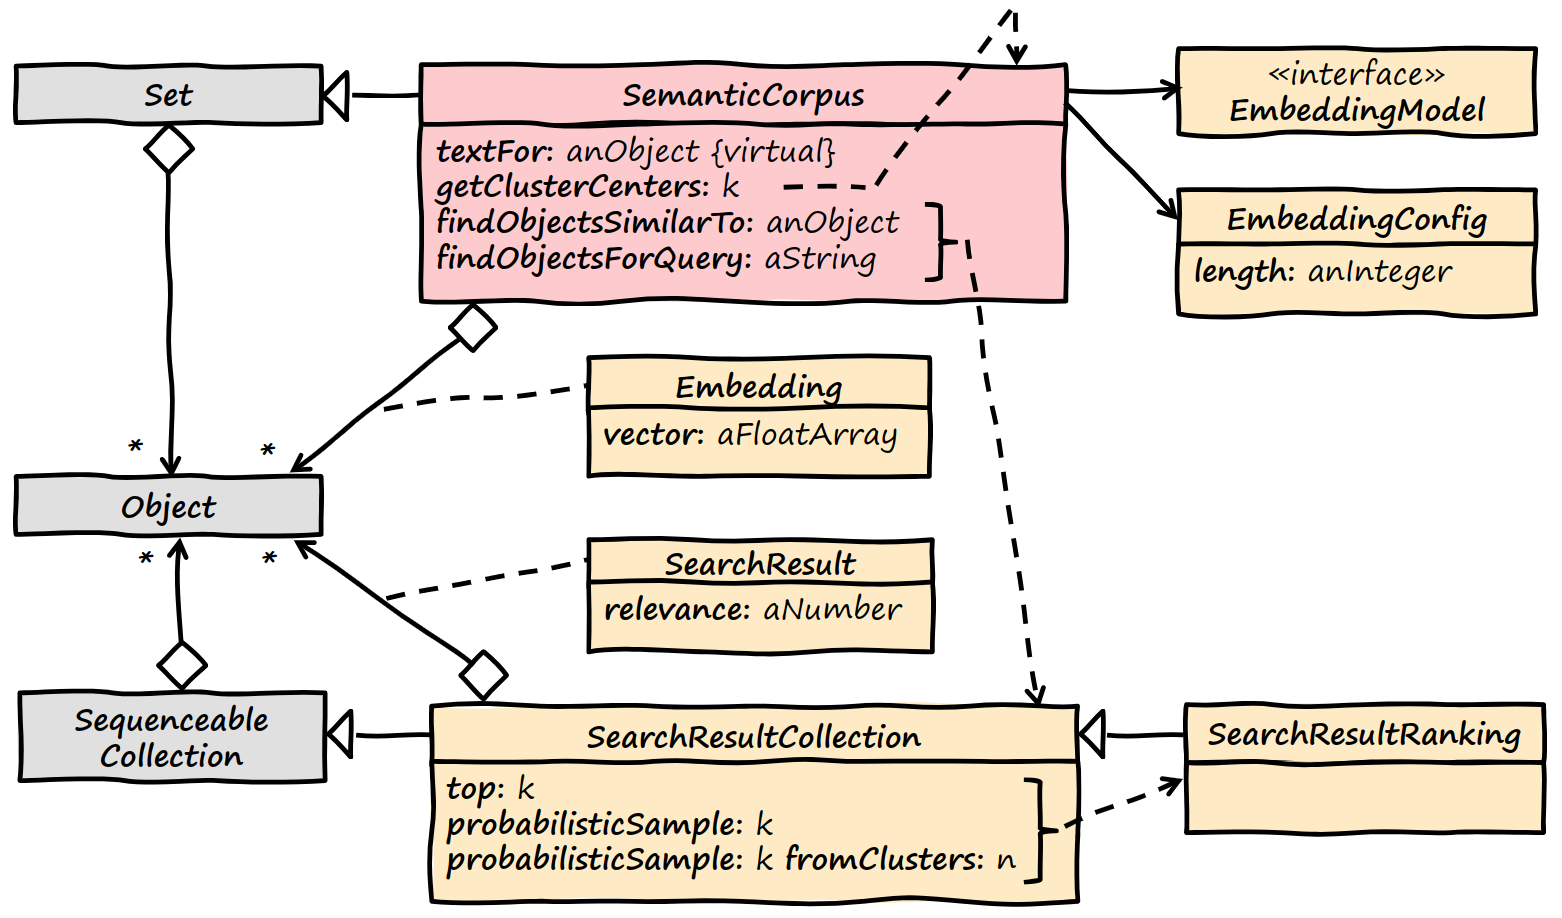
\includegraphics[width=\textwidth]{01_model/search.png}
	\caption[The general object model for semantic search in \semtex.]{
		The general object model for semantic search in \semtex (UML class diagram with Smalltalk-styled method signatures; default multiplicities are $1$; dashed arrows indicate the return class of message sends).
		Programmers can use the entry class \code{SemanticCorpus} (\bold{\textcolor[HTML]{c00000}{red}}) to index domain objects with an embedding model and search, rank, or cluster them.
	}
	\label{fig:semtex/model/search}
\end{figure}

For each object, the corpus computes and stores an \code{embedding} vector that is represented by a \code{FloatArray}, allowing for efficient comparison, memory consumption, and serialization.
To compute embeddings, the corpus is provided with an \code{EmbeddingModel} (which may be implemented by different providers, see \cref{sec:semtex/providers}) and an \code{EmbeddingConfig} for controlling the embedding properties such as the length of embedding vectors.
To embed non-textual object elements, the corpus can be provided with a \emph{text conversion} function through composition or specialization (e.g., by registering an evaluable block or overriding a method)\footnote{Currently accessible through \code{SemanticPluggableCorpus}.}.

The semantic corpus provides methods for searching objects that are \emph{similar} to a reference object or to a natural-language \emph{query} string.
For each search, it answers a \code{SearchResultSet}, which contains a \emph{relevance score} for each object in the corpus\footnote{At the time of writing, these classes have not yet been extracted from the \code{SemanticCorpus} in our public implementation.}.
A result set can be \emph{ranked} into a \code{SearchResultRanking} of a finite length using the different ranking methods discussed in \cref{sec:suggestions/ranking}, such as top-k selection and probabilistic sampling.
Additionally, the semantic corpus also supports cluster-based selection of representative objects without a reference object.

\begin{example}[5]
	A programmer wants to find classes in the system that implement means for semantic search.
	For this, they can create a semantic corpus of all classes based on their names and comments, perform a search, and rank the results:

	\begin{multicode}
		corpus := self \stKeyword{systemNavigation} \stKeyword{allClasses} \newline
		\null\qquad	\stKeyword{asSemanticCorpusWithTitle:} \stSymbol{\#name} \newline
		\null\qquad	\stKeyword{content:} \stSymbol{\#comment}. \newline
		results := corpus \stKeyword{findObjectsForQuery:} \stString{\textquotesingle semantic search database\textquotesingle}. \newline
		ranking := results \stKeyword{top:} \stNumber{5}. \newline
		ranking \printit{\footnote{We use the notation \code{<expr> \printit{<result>}} to indicate a \emph{print-it} evaluation~\cite[p. 13]{thiede2023squeak}.} a SearchResultRanking(\allowbreak\#SemanticCorpus->0.533 \#SemanticHelpSearchTopic->0.442 \#SemanticText->0.385 \#SemanticAgentParser->0.364 \#SemanticMathAgent->0.338)}
	\end{multicode}
\end{example}

\FloatBarrier

\subsection*{Conversations}
\label{sec:semtex/model/conversations}

To support text generation and machine reasoning, we integrate different conversational LLMs into \semtex.
For this, the framework defines a \code{SemanticConversation} class~(\cref{fig:semtex/model/conversation}).
A conversation consists of a sequence of \code{Message}s each of with is specified with a \code{role} (either system, user, or assistant) and a \code{text}.
A programmer can set up a conversation with a sequence of initial messages, such as a system message for providing instructions and a user message for the first question of the user, and ask the conversation to complete itself, which will request the (stateless) LLM and append a new generated assistant message to the conversation.

\begin{figure}
	\centering
	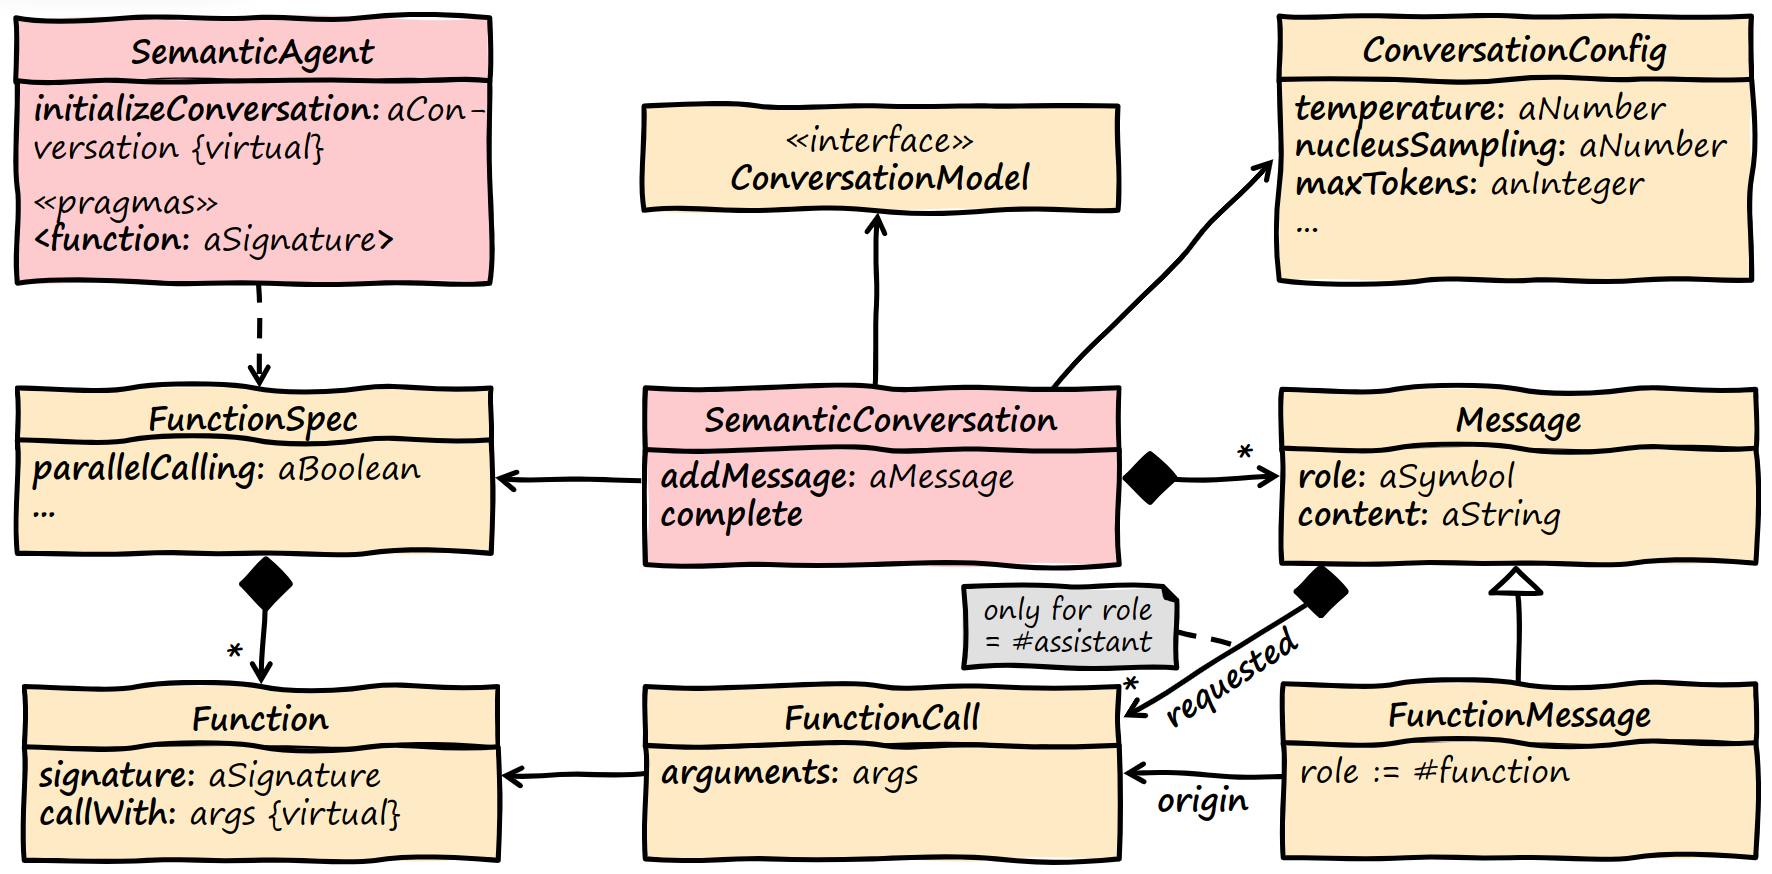
\includegraphics[width=\textwidth]{01_model/conversation.png}
	\caption[The general object model for conversational agents in \semtex.]{
		The general object model for conversational agents in \semtex (UML class diagram with same semantics as before).
		Programmers can create a \code{SemanticConversation} (\bold{\textcolor[HTML]{c00000}{red}}) with a set of messages and request an answer from a conversation model or implement an \code{Agent} class (\bold{\textcolor[HTML]{004080}{blue}}) and declare callable functions via pragmas on it.
	}
	\label{fig:semtex/model/conversation}
\end{figure}

To allow for the construction of agents, the conversation can also be equipped with a \code{FunctionSpec} that provides one or multiple \code{Function}s.
Each function has a name, can specify an optional list of arguments and their constraints as well as a description, and contains an action object (e.g., a block).
When the LLM is invoked, it can issue one or multiple \code{FunctionCall}s based on the function specification as part of the generated assistant message.
The conversation automatically resolves these function calls by \code{call}ing each issued function with the generated arguments, storing the result in a new \code{FunctionMessage}, and providing all function messages to the LLM in another request, which uses the results for generating the next assistant message.

Analogously to semantic corpora, each conversation is configured through a \code{ConversationModel} reference and a \code{ConversationConfig} for controlling the generation behavior through parameters such as the model temperature and the maximum number of tokens to generate.

\begin{example}
	A programmer wants to create a chatbot that can retrieve the current time and date.
	For this, they define a conversation with an appropriate configuration for the LLM, define the necessary functions, and provide the question of the user:

	\begin{multicode}
		\stGlobal{SemanticConversation} \stKeyword{new} \n
		\t	\stKeyword{withConfigDo:} [:\stBlockArg{config} | \n
		\t	\t	\stBlockArg{config} \stKeyword{temperature:} \stNumber{0.2}]; \n
		\t	\stKeyword{addFunction:} \stSymbol{\#getTime} \stKeyword{action:} [\stGlobal{Time} \stKeyword{now}]; \n
		\t	\stKeyword{addUserMessage:} \stString{\textquotesingle What time is it?\textquotesingle}; \n
		\t	\stKeyword{getAssistantReply} \printit{\textquotesingle The current time is 13:59.\textquotesingle}
	\end{multicode}
\end{example}

Additionally, \semtex supports the construction of class-based agents by providing the base class \code{SemanticAgent} which users can specialize to provide custom instructions and functions.
The \code{SemanticAgent} class provides a custom DSL (domain-specific language) for specifying function signatures with its arguments, their constraints, and their descriptions through method pragmas.
The agent class will automatically dispatch function calls and handle errors from called functions.

\begin{example}
	A programmer wants to build a chatbot that can access the running Squeak image to assist the user.
	To achieve this, they create a subclass of \code{SemanticAgent}, initialize the conversation, and define an \code{\#eval:} method:

	\begin{multicode}
		\stGlobal{SemanticAgent} \stKeyword{subclass:} \stSymbol{\#SemanticSqueakAgent} \n
		\t	\stKeyword{instanceVariableNames:} \stString{\textquotesingle\textquotesingle} \n
		\t	\stKeyword{classVariableNames:} \stString{\textquotesingle\textquotesingle} \n
		\t	\stKeyword{poolDictionaries:} \stString{\textquotesingle\textquotesingle} \n
		\t	\stKeyword{category:} \stString{\textquotesingle SemanticText-Model-Agents\textquotesingle} \n
		\n
		SemanticSqueakAgent>>\stSignature{initializeConversation: \stArg{aConversation}} \n
		\t	\stSuper{super} \stKeyword{initializeConversation:} \stArg{aConversation}. \n
		\t	\stArg{aConversation} \stKeyword{addSystemMessage:} \stString{\textquotesingle You are a Squeak"/Smalltalk assistant.\textquotesingle}. \n
		%\t	\stArg{aConversation} \stKeyword{addAssistantMessage:} \stString{\textquotesingle Hi, how can I help you?\textquotesingle}. \n
		\n
		SemanticSqueakAgent>>\stSignature{eval: \stArg{aString}} \n
		\t	\stComment{\textquotedbl Evaluate a Smalltalk expression in the running Squeak image.\textquotedbl} \n
		\t	<\stPragmaKeyword{function:} \stString{eval}( \n
		\t	\t	\stArg{expression:} string \stComment{\textquotedbl %examples: \n
		%\t	\t	- \textquotesingle DateAndTime now\textquotesingle \n
		%\t	\t	- \textquotesingle| collection | collection := 1 to: 10. collection inject: 0 into: [:a :b | a + b]\textquotesingle \n
		%\t	\t	\textquotedbl} \n
		e.g. \textquotesingle (8 nthRoot: 3)-1\textquotesingle\textquotedbl} \n
		\t	)> \n
		\t	\stReturn{\textasciicircum{}} \stGlobal{Compiler} \stKeyword{evaluate:} \stArg{aString}
	\end{multicode}

	Finally, the programmer invokes the agent:

	\begin{multicode}
		\stGlobal{SemanticSqueakAgent} \stKeyword{makeNewConversation} \n
		\t	\stKeyword{addUserMessage:} \stString{\textquotesingle how many windows are open\textquotesingle}; \n
		\t	\stKeyword{getAssistantReply} \printit{\textquotesingle You currently have 138 open windows in your Squeak environment.\textquotesingle}
	\end{multicode}
\end{example}
